\documentclass[11pt]{article}
\usepackage[margin=1in]{geometry}
\usepackage[T1]{fontenc}
\usepackage{lmodern,microtype,amsmath,amssymb,amsthm,mathtools,booktabs,graphicx}
\usepackage[round,authoryear]{natbib}
\usepackage[hidelinks]{hyperref}
\usepackage{enumitem}
\setlist{nosep,leftmargin=*}
\usepackage{fancyhdr}
\pagestyle{fancy}\fancyhf{}\fancyhead[L]{\small Search or Refresh?}\fancyhead[R]{\small Research draft}\fancyfoot[C]{\thepage}
\setlength{\headheight}{14pt}
\newtheorem{theorem}{Theorem}
\newtheorem{proposition}[theorem]{Proposition}
\newtheorem{lemma}[theorem]{Lemma}
\newtheorem{corollary}[theorem]{Corollary}
\newtheorem{remark}[theorem]{Remark}
\newcommand{\E}{\mathbb E}\newcommand{\Prb}{\mathbb P}\newcommand{\R}{\mathbb R}
\newcommand{\TV}{\operatorname{TV}}\newcommand{\spn}{\operatorname{span}}
\newcommand{\supp}{\operatorname{supp}}\newcommand{\cT}{\mathcal T}
\newcommand{\cF}{\mathcal F}\newcommand{\cC}{\mathcal C}
\newcommand{\pos}[1]{\left[#1\right]_+}
\DeclareMathOperator*{\argmax}{arg\,max}
\title{\vspace{-1.2em}\textbf{Search or Refresh?}\\Candidate-Exposure Certificates for\\Offline Policy Extraction}
\author{Anonymous research draft}
\date{September 2026}
\begin{document}
\maketitle
\begin{abstract}
Increasing candidate-action search changes the continuation policy that a critic must evaluate. We study this mismatch separately from ordinary estimation error and develop decision-sensitive certificates for reusing or refreshing a critic. A finite-horizon construction exhibits declining return with more search despite an exact reference-policy critic; a delayed version requires a prescribed number of synchronous local backups to reverse the consequential ranking. Our central result computes, without enumerating candidate sets, the expected worst ranking loss allowed by an interval box. This menu-wise envelope is within a factor of four of the worst loss of a single fixed value vector, and is exact with two actions. Combining it with budget-matched Bellman residuals yields finite-data stopping certificates whose validity survives adaptive reuse of one offline dataset. A separate advantage-based gate certifies policy replacement, while a two-environment lower bound identifies uncertainty that unlimited computation cannot remove. CPU experiments validate the formulas and expose important limitations: candidate-sensitive stopping reduces backup calls by 52.7\% on a controlled rare-choice family but only 5.2\% on random graphs, where diagnostic overhead overwhelms the saving. Conservative selection rejects harmful low-coverage proposals but can substantially delay useful improvements. Fitted linear critics further show that refresh is not uniformly beneficial. The results characterize what larger search budgets require a critic to know, rather than establish a universally efficient search--refresh scheduler.
\end{abstract}

\section{Introduction}
Policy extraction is an important component of offline reinforcement learning (RL): a useful value function does not automatically produce a useful executable policy \citep{park2024bottleneck}. One simple extractor samples $K$ actions from a fixed proposal $\beta(\cdot\mid s)$ and chooses the action with the largest critic score. Larger $K$ exposes more supported alternatives, but also changes the downstream behavior under which an upstream action should be valued. Training a critic for one continuation policy and deploying another therefore creates a potential mismatch even before estimation error is considered.

This issue is not the discovery of a new Bellman operator. Expected-max Q-learning (EMaQ) already defines the budget-dependent operator and establishes properties of its fixed points \citep{ghasemipour2021emaq}. Nor is the general tradeoff between policy improvement and evaluation new \citep{scherrer2015ampi}. We ask a narrower question: \emph{given a partly refreshed critic and uncertainty about its target values, which of its unresolved errors can the intended candidate budget actually expose?}

The relevant event is not merely ``the critic is inaccurate.'' Two actions must appear together, the extractor must select the wrong one, and better-ranked candidates must fail to screen the error. This suggests weighting uncertain pairwise rankings by their candidate-set exposure. The resulting certificate is zero when $K=1$, can increase or decrease with $K$, and can be much smaller than a norm-based value-error certificate.

Our central mathematical contribution is a closed-form interval envelope for this exposure, including a constant-factor relationship to the fixed-vector robust loss. We connect it to finite-horizon return, budget-matched residuals, and a simultaneous offline model confidence event. Exact constructions separate the cost of propagating changed continuation values from irreducible statistical ambiguity. Experiments deliberately include negative controls and complete diagnostic accounting: fewer Bellman sweeps need not mean less work, and an interval guarantee may be statistically valid yet practically conservative.

\paragraph{Scope.} We analyze finite action sets, known fixed proposals, independent one-step offline samples, and known time-layer support. The main stopping routine chooses refresh work for a \emph{specified} budget $K$. A sequential candidate-selection wrapper is safe but is not claimed optimal over all $(K,m)$ allocations. The local-sweep construction is not a computational lower bound against backward dynamic programming or arbitrary model-based planning.

\section{Setup and an exact mismatch}
Consider a finite-horizon MDP with nonterminal layers $\mathcal S_0,\ldots,\mathcal S_{H-1}$, an absorbing terminal state, initial distribution $\mu$ on $\mathcal S_0$, rewards in $[0,1]$, and discount $\gamma\in(0,1]$. Nonterminal transitions advance exactly one layer; earlier termination is allowed. We suppress the layer index when it is determined by the state. Actions outside $\supp\beta(\cdot\mid s)$ are irrelevant to the extractor. The illustrative opening example rescales rewards by ten; all statistical experiments use $[0,1]$ rewards.

Let $C=(A_1,\ldots,A_K)$ contain independent draws from $\beta$. A fixed action-index priority resolves equal scores. Write $I_q(C)$ for the highest-priority maximizer of $q$ in $C$, $\pi_{q,K}$ for its marginal action distribution, and
\begin{equation}
 \cF_K q(s)=\E_C\max_{a\in C}q(s,a),\qquad
 \cT_K q(s,a)=r(s,a)+\gamma P_{s,a}\cF_Kq.
 \label{eq:operator}
\end{equation}
This is the EMaQ operator \citep{ghasemipour2021emaq}. Its finite-horizon solution $Q_K$ is obtained by backward induction; $V_K=\cF_KQ_K$ and $\pi_{Q_K,K}$ are optimal among policies that observe the independently drawn menu and must choose from it. Their benchmark is \emph{not} unrestricted optimal control $Q^*$.

\subsection{More search can hurt an exact baseline critic}
At a root state, Safe pays $c$ and terminates, while Continue leads to a final state. At that state, Good pays $B$ and Bad pays zero. The proposal chooses Safe with probability $\sigma$ and Good with probability $p$. Assume $Bp<c$. The exact baseline critic ranks Safe above Continue. Best-of-$K$ under this frozen critic has value
\begin{equation}
 J_{\rm fr}(K)=c\{1-(1-\sigma)^K\}+(1-\sigma)^K B\{1-(1-p)^K\}.
 \label{eq:fork}
\end{equation}
For $(c,B,p,\sigma)=(2,10,.1,.1)$, this becomes
$2+8(.9)^K-10(.9)^{2K}$. It is $1.10$ at $K=1$, approximately $3.59$ at $K=8$, $2.26$ at $K=32$, and approaches $2$. One budget-matched backup instead values Continue at $10(1-.9^K)$; at $K=32$ the resulting return is approximately $9.66$.

The frozen critic is exact for $Q^\beta$, not for the deployed continuation. These returns do not contradict improvement over $\beta$: nonmonotonicity is between different extracted policies, and the baseline return is only $1.10$.
\begin{figure}[t]
 \centering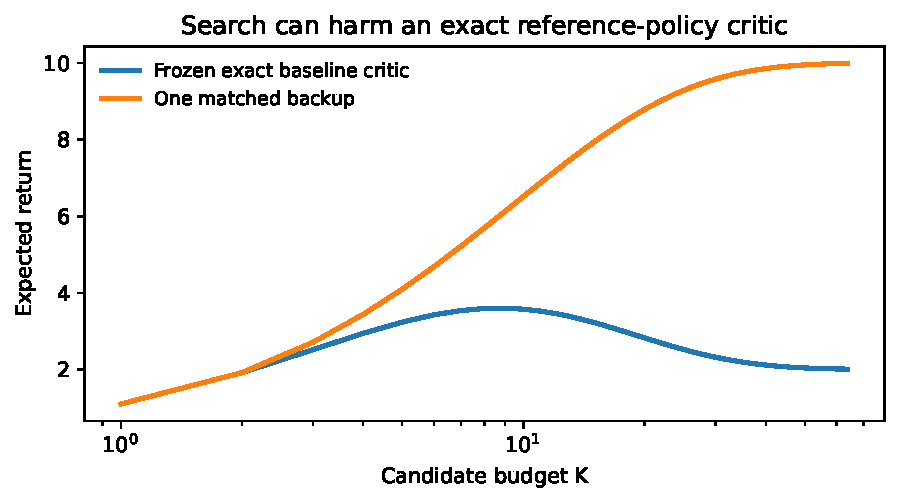
\includegraphics[width=.79\linewidth]{../figures/opening_fork.pdf}
 \caption{An exact reference-policy critic can become a poor ranking rule as the candidate budget changes. Rewards are rescaled here for readability. The refresh curve includes one exact matched backup, but this figure is not a matched-compute comparison.}
 \label{fig:fork}
\end{figure}

\begin{theorem}[Exact local propagation cost]\label{thm:delay}
Insert forced-action states so that Continue reaches the final choice after $d$ transitions. Let $R_K=\gamma^dB(1-(1-p)^K)$ and assume $\gamma^dBp<c<R_K$. Initialize $q_0=Q^\beta$ and apply synchronous sweeps $q_{m+1}=\cT_Kq_m$. For $m<d$ the root retains its original ranking; at $m=d$ it has the matched ranking. For every $m<d$,
\begin{equation}
 J_K-J(\pi_{q_m,K})=
 \underbrace{\{1-\sigma^K-(1-\sigma)^K\}}_{\text{both root actions appear}}(R_K-c),
 \label{eq:delay}
\end{equation}
and the gap is zero for $m\ge d$.
\end{theorem}
The theorem gives an exact cost for this \emph{specified synchronous recurrence}. A known layered model can propagate information backward in one ordered pass, so there is no claim that every planner needs $d$ full sweeps. This distinction is central to our compute accounting.

\section{Candidate-exposure certificates}
At a fixed state, sort actions in increasing critic order, including the fixed tie priority, and index them by $1,\ldots,A$. Let $\beta_i$ be their proposal probabilities and $F_i=\sum_{j\le i}\beta_j$, with $F_0=0$. The extractor's selection probabilities are
\begin{equation}
 w_i(K)=\Prb\{I_q(C)=i\}=F_i^K-F_{i-1}^K.
 \label{eq:weights}
\end{equation}
For a possible true value vector $v$ define its one-state ranking loss
\begin{equation}
 \ell_K(q,v)=\E_C\{\max_{a\in C}v_a-v_{I_q(C)}\}
 =\cF_Kv-\sum_iw_i(K)v_i.
 \label{eq:local-loss}
\end{equation}
The loss is nonnegative, and vanishes identically for $K=1$.

Suppose $v$ is only known to belong to a rectangular box $[l,u]$. Two robust quantities must not be confused:
\begin{align}
 R_K(q;l,u)&=\sup_{v\in[l,u]}\ell_K(q,v),\label{eq:robust}\\
 \Gamma_K(q;l,u)&=\E_C\sup_{v\in[l,u]}
 \{\max_{a\in C}v_a-v_{I_q(C)}\}.\label{eq:envelope}
\end{align}
The first uses one value vector for every menu. The second allows the adverse vector to change with the menu and is therefore an upper bound. We compute the latter without enumerating $A^K$ menus.

\begin{theorem}[Closed-form menu envelope]\label{thm:envelope}
Let $D_{ij}=(u_j-l_i)_+$ for $j<i$, and define
\begin{equation}
 B_i(t)=\sum_{j<i:\,D_{ij}>t}\beta_j,\qquad
 H_i(t)=F_i^K-F_{i-1}^K-(F_i-B_i(t))^K+(F_{i-1}-B_i(t))^K.
 \label{eq:tail}
\end{equation}
Then
\begin{equation}
 \Gamma_K(q;l,u)=\sum_i\int_0^\infty H_i(t)\,dt.
 \label{eq:integral}
\end{equation}
The expression is computable in $O(A^2\log A)$ arithmetic/sort work and $O(A)$ additional memory. Furthermore,
\begin{equation}
 \frac14\Gamma_K(q;l,u)\le R_K(q;l,u)\le\Gamma_K(q;l,u).
 \label{eq:factor}
\end{equation}
For two supported actions, in increasing $q$ order,
\begin{equation}
 R_K=\Gamma_K=(u_1-l_2)_+\{1-\beta_1^K-\beta_2^K\}.
 \label{eq:two-action}
\end{equation}
\end{theorem}
\paragraph{Interpretation.} $H_i(t)$ is the probability that $i$ is selected and a lower-ranked action with interval-implied loss above $t$ appears in the same menu. The four powers in \eqref{eq:tail} account for both co-occurrence and screening by higher-ranked actions. The theorem's factor four is a proved upper factor, not claimed the best universal constant. It compares two \emph{local box-relaxed} quantities; it does not assert minimax optimality over Bellman-consistent MDPs.

\paragraph{Why the quantifiers matter.} With three equiprobable actions, $K=3$, $q_1<q_2<q_3$, and all intervals $[0,1]$, direct calculation gives $\Gamma_K=8/9$ but $R_K=2/3$. Reporting the former as the exact fixed-critic worst case would be incorrect.

\paragraph{Search can screen errors.} Take $q=(0,1,3)$, true values $v=(1,0,3)$, and a uniform proposal. Only the first two actions are inverted; the third is correctly ranked and dominates both. Then
\begin{equation}
 \ell_K(q,v)=(2/3)^K-2(1/3)^K.
 \label{eq:screen}
\end{equation}
It initially increases but tends to zero. A generic statement that larger $K$ always exposes more ranking damage is therefore also false.

\subsection{From local uncertainty to return}
\begin{theorem}[Exact loss propagation]\label{thm:performance}
Fix $q$, $K$, and $\pi=\pi_{q,K}$. Let $\ell(s)=\ell_K(q(s,\cdot),Q_K(s,\cdot))$. Then
\begin{equation}
 V_K(s)-V^\pi(s)=\ell(s)+\gamma P^\pi_s(V_K-V^\pi).
 \label{eq:resolvent}
\end{equation}
If $Q_K(s,\cdot)\in[l_s,u_s]$ for all supported actions, then
\begin{equation}
 0\le J_K-J(\pi)\le
 \E_\pi\sum_{h=0}^{H-1}\gamma^h\Gamma_K(q(S_h,\cdot);l_{S_h},u_{S_h})
 \le\sum_{h=0}^{H-1}\gamma^h\max_{s\in\mathcal S_h}\Gamma_K(q_s;l_s,u_s).
 \label{eq:performance}
\end{equation}
Terms after termination are zero.
\end{theorem}
This separates two sources of conservatism: a local rectangular envelope and a worst-state occupancy bound. The latter avoids estimating a deployment occupancy distribution. When the true model is known, the middle expression can instead be evaluated by backward recursion; experiments use the final, more conservative expression for stopping.

\section{Finite data and adaptive critic reuse}
An offline dataset supplies $n(s,a)$ independent one-step reward/transition samples per state--action pair. Counts are fixed independently of outcomes. Rewards are Bernoulli, proposals are known, and each row has a known successor support of size $D_{s,a}$, including termination. This setting is intentionally narrower than arbitrary behavior trajectories.

Let $M$ be the number of state--action rows. Use a two-sided exact binomial reward interval $[r^-_{s,a},r^+_{s,a}]$ with per-row failure probability $\delta/(2M)$. For empirical transition row $\widehat P_{s,a}$ use a total-variation radius
\begin{equation}
 t_{s,a}=\min\left\{1,\sqrt{\frac{D_{s,a}\log 2+\log(2M/\delta)}{2n(s,a)}}\right\}.
 \label{eq:tv-radius}
\end{equation}
An unsampled row receives the full reward interval and simplex; a one-point successor support has radius zero. A union bound gives one event $\mathcal E$ of probability at least $1-\delta$ on which the true model belongs to every row confidence set. This event concerns the model, not a list of already chosen critics, and therefore permits subsequent adaptive reuse.

\subsection{Residual bands with a statistical floor}
For any data-dependent $q$ and integer $K$, let $v_q=\cF_Kq$, including terminal value zero, and
\begin{align}
 e_{s,a}(q,K)&=\max\{\widehat r_{s,a}-r^-_{s,a},r^+_{s,a}-\widehat r_{s,a}\}
 +\gamma t_{s,a}\spn(v_q\mid\supp P_{s,a}),\label{eq:model-error}\\
 d_h(q,K)&=\max_{s\in\mathcal S_h,\,a\in\supp\beta_s}
 \{|\widehat\cT_Kq(s,a)-q(s,a)|+e_{s,a}(q,K)\},\label{eq:residual}\\
 b_H&=0,\qquad b_h=d_h+\gamma b_{h+1}.\label{eq:radius}
\end{align}
\begin{theorem}[Uniform residual and stopping certificate]\label{thm:stopping}
On $\mathcal E$, simultaneously for all finite data-dependent critics $q$ and all $K\ge1$,
\begin{equation}
 |Q_K(s,a)-q(s,a)|\le b_h\quad(s\in\mathcal S_h,\ a\in\supp\beta_s).
 \label{eq:band}
\end{equation}
Consequently the bound in \eqref{eq:performance}, evaluated with $l_s=q_s-b_h$ and $u_s=q_s+b_h$, certifies return loss at most $\varepsilon$ whenever it is at most $\varepsilon$. This remains valid at an adaptively chosen stopping time, after querying any number of search budgets and refresh iterates using the same dataset. For these symmetric boxes, it never exceeds the generic bound $2\sum_h\gamma^hb_h$.
\end{theorem}
Small empirical residual does not imply small uncertainty: the $e_{s,a}$ terms remain even at the empirical fixed point. Conversely, if no consequential pair can be misranked, the exposure certificate can vanish while some value radii remain positive. Action-gap sensitivity is a classical principle \citep{farahmand2011gap}; the additional object here is the candidate-budget-dependent exposure of uncertain gaps.

\paragraph{Stopped refresh.} Starting from an empirical baseline critic $q_0$, compute $\widehat\cT_Kq_m$ and use that same result both as the diagnostic residual and, if needed, the next iterate. Stop at the first certificate below $\varepsilon$, or at a specified update cap. An $m$-update returned critic has incurred $m+1$ backup calls, because its final diagnostic also costs a backup. The exact envelope incurs additional pair/sort work. An uncertified capped iterate is explicitly marked uncertified; it is not silently declared successful.

\subsection{Safe replacement is a different guarantee}
Being close to the $K$-matched optimum and improving on the current policy are different claims. For replacement we bound $Q^{\pi_o}$, where $\pi_o$ is the retained policy, by robust backward evaluation over the same model confidence set. Given a proposed policy $\pi_n$, define
\begin{equation}
 G(s)=\sum_{a:\Delta\pi(a)\ge0}\Delta\pi(a)L_o(s,a)
      +\sum_{a:\Delta\pi(a)<0}\Delta\pi(a)U_o(s,a),
 \quad \Delta\pi=\pi_n-\pi_o.
 \label{eq:gate}
\end{equation}
\begin{proposition}[Adaptive conservative replacement]\label{prop:gate}
$G(s)$ is exactly the minimum of $\langle\Delta\pi(s),v\rangle$ over $v\in[L_o(s),U_o(s)]$. On $\mathcal E$, either of the following suffices for $J(\pi_n)\ge J(\pi_o)$: (i) $G(s)\ge0$ at every state; (ii) a robust lower bound on $J(\pi_n)$ is at least a robust upper bound on $J(\pi_o)$. A sequence retaining the previous policy whenever both tests fail is nondecreasing in true return on this same event, even when proposals and budgets are chosen adaptively.
\end{proposition}
This is a conservative policy-improvement construction, not a claim to originate safe offline improvement \citep{laroche2019spibb}. Test (i) cancels statewise value offsets because $\sum_a\Delta\pi(a)=0$, but can reject beneficial joint downstream changes. Test (ii) can recover some of them at the cost of additional robust evaluation. Rejection proves neither harm nor impossibility of improvement.

\section{An information limit on additional computation}
\begin{theorem}[Search-exposed statistical ambiguity]\label{thm:stat}
Consider one state with two actions, proposal probabilities $(1/2,1/2)$, a known safe mean $1/2$, and an unknown risky Bernoulli mean $1/2\pm\Delta$, where $0<\Delta\le1/4$. The offline dataset contains $n$ risky-action samples. For any possibly randomized extractor with unlimited computation that must choose from its $K$-sample menu, if $n\le1/(32\Delta^2)$, at least one of the two environments has expected regret relative to its matched-$K$ optimum at least
\begin{equation}
 \frac{\Delta}{4}\chi_K,\qquad \chi_K=1-2^{1-K}.
 \label{eq:stat-lower}
\end{equation}
\end{theorem}
The multiplier is the same co-occurrence probability as in the exact two-action certificate. Choosing $\Delta=(32n)^{-1/2}$ gives an order-$\chi_K/\sqrt n$ obstruction. The result holds for fixed $K$; it does not prevent choosing $K=1$, for which both the comparator and the ranking requirement are different and the bound is zero. It also does not turn failure of a particular certificate into an impossibility result for a particular dataset.

\section{Experiments}
\label{sec:experiments}
All core experiments are CPU-only and use exact policy evaluation, removing rollout noise from measured returns. Candidate menus are integrated analytically; tiny independent enumeration checks verify that implementation. Learners receive empirical models or fixed feature maps, never the true values used to audit them. All parameter grids, data-generation assumptions, primitive work counts, and raw scientific CSVs accompany the manuscript.

\subsection{Formula and construction checks}
We check 400 interval geometries with two to five actions and five candidate budgets, enumerate 5,840 menus on the small-budget subset, and enumerate 6,000 interval vertices for the exact fixed-vector robust comparator. The largest envelope/enumeration discrepancy is $1.78\times10^{-15}$; the largest observed $\Gamma_K/R_K$ ratio is $1.877$, consistent with (but not establishing sharpness of) the factor-four theorem. The fork grid contains 2,952 $(d,p,\sigma,K,m)$ configurations, including cases without an initial ranking mismatch. All exact propagation predictions tested agree to numerical precision.

\subsection{Refresh work: a positive family and a negative family}
We compare exposure stopping to generic residual stopping, both with paid diagnostic backups. On 234 random graph--budget configurations (horizons $3,6,10$, two states per layer, and $2,8$, or $32$ actions), tolerance $.02$, mean backup calls fall only from $6.150$ to $5.829$. The exact certificate's operation proxy is $4.134$ times the generic proxy: quadratic pair work overwhelms the 5.2\% backup saving. Both methods happen to return matched-optimal policies in this grid; they are conservative relative to the first acceptable oracle iterate.

On a controlled rare-downstream-choice grid of 180 configurations, mean calls fall from $5.994$ to $2.833$ (52.7\%). Under the same explicit proxy, total work falls by 48.0\%. This family often makes changed continuation values irrelevant to the root ranking, which is exactly when norm-only convergence is unnecessary. It is a mechanism test, not evidence of a universal speedup.

\begin{table}[t]
\centering\small
\begin{tabular}{lrrrr}
\toprule
Family & Configurations & Generic calls & Exposure calls & Proxy ratio\\
\midrule
Random stochastic graphs & 234 & 6.150 & 5.829 & 4.134\\
Rare downstream choices & 180 & 5.994 & 2.833 & 0.520\\
\bottomrule
\end{tabular}
\caption{Exposure/generic proxy ratio includes pairwise diagnostic work; below one is better. Baseline critic construction is shared. This is not a wall-clock or hardware-independent FLOP claim.}
\label{tab:work}
\end{table}
A cheap tabular backward-DP baseline solves the matched empirical problem in one ordered pass. It is stronger computationally than the synchronous methods here. Starting with exact empirical $Q^\beta$, $H-1$ unmonitored sweeps also suffice for full propagation; a diagnostic method is not automatically cheaper. The experiment therefore supports selective savings \emph{within a local-update/certification workflow}, not superiority over tabular planning.

\subsection{Finite-data selection and its conservatism}
Four families (depth-one and depth-four forks, three- and five-layer stochastic graphs), four per-state data budgets ($200$ to $200{,}000$), and 30 seeds per condition produce 480 offline dataset instances. Three budget proposals per dataset yield 1,440 sequential replacement tests. At $\delta=.05$ per dataset, 907 proposals are accepted and 445 receive a $.03$ matched-optimality certificate. We observe one model-confidence failure, but no false replacement or false near-optimality certificate. These observations are not a substitute for the probability guarantee, and the three tests on a dataset are not independent trials.

The confidence method can be very conservative. On stochastic five-layer graphs at 2,000 allocated samples per state, none of the 90 proposals is accepted, despite a mean proposed return around $.670$ versus a baseline around $.306$. At 200,000 samples, the acceptance fraction is $.844$. No near-optimality certificate is produced for either stochastic family at the tested budgets: safe improvement and near-optimality are substantially different demands.

\subsection{Estimation-only and function-approximation controls}
A one-step, eight-action control eliminates continuation mismatch. One action has reward mean $.6$ and proposal mass $.9$; the others have mean $.5$ and share the remaining mass. Across 500 datasets and 1,500 proposals, 625 ungated proposals are worse than the current retained policy, while the conservative gate accepts 301 and none is harmful. At 100 allocated samples per state, no proposal is accepted; at 100,000 all are accepted. This negative control prevents attributing all search degradation to continuation mismatch.

Finally, 20 stochastic tasks, three dataset seeds, and three budgets produce 180 small fitted-linear-critic configurations. Each time layer has separate state/action main-effect features plus two random interaction features; weighted ridge fitting leaves within-layer approximation error. Five matched fitted sweeps improve frozen return in 56.1\% of configurations and harm it in 43.9\%; the mean gain is $.00726$. The experiment validates neither a neural scaling law nor a general guarantee for fitted iteration. Instead it demonstrates why exact-model refresh intuition must not be assumed to survive projection.
\begin{figure}[t]
 \centering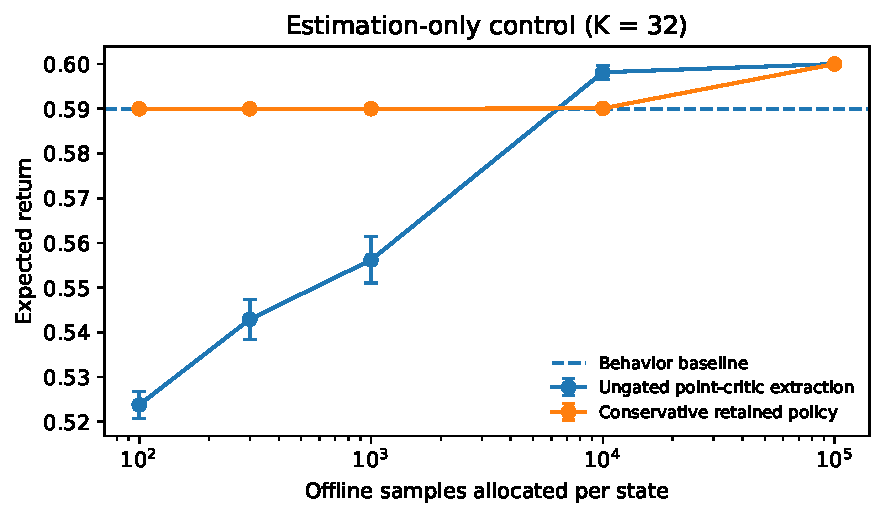
\includegraphics[width=.81\linewidth]{../figures/rare_data.pdf}
 \caption{Low-coverage estimation-only control at $K=32$. Means and pointwise $\pm1.96$ standard errors across 100 independent seeds per sample-size condition. The retained-policy gate trades speed of improvement for conservative protection.}
 \label{fig:data}
\end{figure}

\section{Related work and limitations}
\paragraph{Prior work.} EMaQ supplies the expected-max operator, fixed-point interpretation, and budget monotonicity at the matched solution \citep{ghasemipour2021emaq}; none is claimed new. Approximate modified policy iteration analyzes evaluation/improvement tradeoffs \citep{scherrer2015ampi}. Action-gap theory explains why policy quality may converge before value accuracy \citep{farahmand2011gap}; our interval envelope makes random candidate co-occurrence explicit. Best-of-$N$ alignment analyzes imperfect reward models and pessimistic extraction \citep{huang2025best}, while our exact fork isolates sequential mismatch. Recent decoupled extraction uses frozen behavior proposals and independent critics, and discusses candidate-budget sensitivity \citep{lin2026decoupling}. Offline extraction/generalization bottlenecks \citep{park2024bottleneck} and safe baseline improvement \citep{laroche2019spibb} provide the broader context. The intended distinction is the menu-exposure certificate and its finite-data refresh application, not an assertion that these broader phenomena are previously unknown.

\paragraph{Limitations.} Rectangular value bounds ignore Bellman coupling and shared estimation errors; the factor-four result is only relative to that relaxation. Worst-state propagation can be much looser than occupancy-aware propagation. Exact menu integration presumes a finite enumerable action set and known proposal, whereas large generative policies require additional approximation. The offline guarantee is not established for arbitrary dependent trajectories or learned proposals. Certification and robust evaluation can cost more than the work they save. Large candidate sets in a small table can also be compiled into a categorical policy, bypassing repeated score calls; our inference-cost discussion does not hide this alternative. There is no large-scale continuous-control or neural experiment and no theorem of globally optimal compute allocation. Independent novelty and proof review remain necessary before a submission claim.

\section{Conclusion}
The decision relevance of critic error depends on which alternatives a search budget can place in the same candidate set. A closed-form exposure envelope quantifies that dependence, including screening by better-ranked actions and a constant-factor comparison to fixed-vector worst-case loss. It yields an adaptive finite-data certificate for stopping budget-matched refresh, but computation and information remain distinct: some errors need propagation, some cannot be resolved from the dataset, and some need not be resolved for the intended extractor. The experiments support these distinctions while rejecting a blanket claim that more refresh or more elaborate certification is always worthwhile.

\bibliographystyle{plainnat}
\bibliography{references}
\clearpage
\appendix
\section{Proofs}
\subsection{Expected-max preliminaries}
For any two score vectors $x,y$ and any menu $C$,
$|\max_{a\in C}x_a-\max_{a\in C}y_a|\le\|x-y\|_\infty$.
Averaging proves nonexpansiveness of $\cF_K$. It is also monotone and preserves constant shifts. Backward induction therefore defines a unique finite-horizon $Q_K$. Observing the sampled menu before acting gives the menu maximization in the Bellman optimality recursion; any measurable randomized choice from that menu is no better than its maximizer. This proves the benchmark interpretation used in the main text and is the finite-horizon counterpart of EMaQ's established fixed-point theory.

\subsection{Proof of the fork and Theorem~\ref{thm:delay}}
The frozen root chooses Continue exactly when every sampled action is Continue, an event of probability $(1-\sigma)^K$. The final policy chooses Good whenever at least one Good sample appears, with probability $u_K=1-(1-p)^K$. Multiplying these independent decision probabilities gives \eqref{eq:fork}. With depth $d$ the effective downstream payoff is $R_K=\gamma^dBu_K$.

At the final state, both initial critic entries already equal their immediate rewards, so every later sweep leaves them unchanged. Its matched extracted value, however, is $Bu_K$ rather than $Bp$. One sweep changes the predecessor's continuation score. Inductively, after $m$ synchronous sweeps the correction has reached exactly the states at distance at most $m$ from the final choice; upstream scores have the same uncorrected children as in the previous sweep. Hence for $m<d$ the root Continue score remains $\gamma^dBp$, and at $m=d$ it becomes $R_K$. Forced-action states introduce no other rankings.

Before the switch the return is $c(1-(1-\sigma)^K)+(1-\sigma)^KR_K$. Afterwards it is $c\sigma^K+(1-\sigma^K)R_K$, because Safe is selected only when every root candidate is Safe. Subtraction gives \eqref{eq:delay}. The sign assumptions make the two rankings strict. This argument proves an equality for the prescribed iterates, not an adversarial oracle-complexity theorem.

\subsection{Proof of Theorem~\ref{thm:envelope}}
If $I_q(C)=i$, the menu contains $i$ and no action ranked above $i$. The event has probability $F_i^K-F_{i-1}^K$, proving \eqref{eq:weights}. For that fixed menu,
\begin{equation}
 \sup_{v\in[l,u]}\{\max_{a\in C}v_a-v_i\}
 =\max\bigl(\{0\}\cup\{(u_j-l_i)_+:j\in C,\ j<i\}\bigr).
 \label{eq:point-envelope}
\end{equation}
The upper bound follows coordinatewise. It is attained by setting $v_i=l_i$ and setting the other present coordinates to their upper endpoints. The selected action is determined by $q$, not by this adverse $v$.

Fix $t\ge0$, and let $B_i(t)$ denote the proposal mass of the lower-ranked actions with $D_{ij}>t$. The event that the selected action is $i$ and \eqref{eq:point-envelope} exceeds $t$ requires at least one $i$, at least one such threatening action, and no action above $i$. Starting from the event that $i$ is selected and subtracting the event containing no threat gives exactly $H_i(t)$ in \eqref{eq:tail}. Events for different selected $i$ are disjoint. The nonnegative tail-integral identity yields \eqref{eq:integral}.

For each $i$, sort its at most $i-1$ positive distinct thresholds. Between adjacent thresholds $B_i(t)$ is constant. Accumulate interval length times the four-power probability, updating the threat mass at every threshold. Sorting costs $O(i\log i)$ and scanning $O(i)$, so the total is $O(A^2\log A)$ with one $O(A)$ scratch buffer. Zero-mass actions may be omitted. This counts arithmetic operations on the powers, not bit complexity for unbounded integers $K$.

To prove the upper part of \eqref{eq:factor}, move the supremum inside the expectation. For the lower part, draw one global random vector $Z$ by independently selecting each coordinate's lower or upper endpoint with probability $1/2$. For any fixed menu with positive envelope, choose a maximizing threatening action $j\ne i$. On the event $Z_j=u_j$, $Z_i=l_i$, which has probability $1/4$, the menu's actual loss is at least its envelope. On other events the loss is nonnegative. Thus
\[
 \E_Z\E_C\{\max_{a\in C}Z_a-Z_{I_q(C)}\}\ge\Gamma_K/4.
\]
Every realization $Z$ is one fixed vector in the box, so the left side is at most $R_K$. The argument uses neither Bellman realizability nor independence of coordinates in an actual critic; it only constructs admissible vectors for the rectangular relaxation.

With two actions, loss is possible only when both appear. On that event the selected action is 2 and the loss is $(v_1-v_2)_+$. The same fixed choice $v_1=u_1,v_2=l_2$ maximizes all nonzero-loss menus simultaneously. The probability of both actions is $1-\beta_1^K-\beta_2^K$, proving equality. For verification with small $A$, the function $\ell_K(q,v)$ is convex in $v$ (a maximum averaged over menus minus a linear term). Maximizing a convex function on a rectangle has a vertex maximizer: holding all other coordinates fixed, moving a coordinate to one of its endpoints cannot decrease the maximum. Repeating over coordinates justifies our exhaustive corner comparator.

\subsection{Proof of Theorem~\ref{thm:performance}}
Use $Q_K=r+\gamma PV_K$ and $Q^\pi=r+\gamma PV^\pi$. Adding and subtracting $\sum_a\pi(a\mid s)Q_K(s,a)$ gives
\begin{align*}
 V_K(s)-V^\pi(s)
 &=\cF_KQ_K(s)-\sum_a\pi(a\mid s)Q_K(s,a)
   +\gamma\sum_a\pi(a\mid s)P_{s,a}(V_K-V^\pi)\\
 &=\ell(s)+\gamma P^\pi_s(V_K-V^\pi).
\end{align*}
The first term is the expected regret of using the $q$-selected action in the same random menu whose $Q_K$ maximizer defines $V_K$. This common-menu coupling is essential. Unroll to termination and average under $\mu$ to obtain an exact sum of local losses along $\pi$. Apply Theorem~\ref{thm:envelope} at every state. At each layer, the probability of still being nonterminal is at most one; bounding its contribution by the largest local envelope yields the last expression in \eqref{eq:performance}. Nonnegativity follows either from the local losses or the matched-budget optimality interpretation.

\subsection{Simultaneous model confidence event}
For a fixed transition row with $D$ possible successors, total variation between $\widehat P$ and $P$ equals
$\max_{B\subseteq[D]}\{\widehat P(B)-P(B)\}$.
For each fixed subset $B$, Hoeffding's one-sided inequality for the sample indicators gives
$\Prb\{\widehat P(B)-P(B)>t\}\le e^{-2nt^2}$.
A union bound over at most $2^D$ subsets and the radius in \eqref{eq:tv-radius} gives failure at most $\delta/(2M)$. Clipping the radius at one covers every simplex point. When $D=1$ there is no transition uncertainty. The binomial interval has failure at most $\delta/(2M)$ by inversion of its two equal-tail binomial tests. Union bounding both kinds of intervals over $M$ rows gives $\Prb(\mathcal E)\ge1-\delta$.

This proof conditions on fixed outcome-independent counts. It does not justify treating dependent transitions from an arbitrarily stopped trajectory as independent samples. Our data generator draws binomial reward and multinomial successor counts directly, exactly the sufficient statistics of the declared independent experiment. The aggregate representation avoids storing hundreds of thousands of redundant one-step records without changing their distribution.

\subsection{Proof of Theorem~\ref{thm:stopping}}
On $\mathcal E$, for any finite vector $v$ on a row's support,
\[
 |(P-\widehat P)v|\le \TV(P,\widehat P)\spn(v).
\]
To see this, subtract the midpoint of the minimum and maximum of $v$, use that $(P-\widehat P)\mathbf1=0$, and apply the $\ell_1$--$\ell_\infty$ inequality. Reward containment and this inequality imply
$|\cT_Kq-\widehat\cT_Kq|\le e(q,K)$ simultaneously for every $q,K$. The implication is deterministic on a model-containment event; $q$ need not be independent of the data.

At the final layer, there is no continuation, so the residual triangle inequality gives $|Q_K-q|\le d_{H-1}=b_{H-1}$ on supported actions. Assuming the bound at layer $h+1$, nonexpansiveness of $\cF_K$ on the proposal support implies
\[
 |Q_K(s,a)-q(s,a)|
 \le |\cT_Kq(s,a)-q(s,a)|+\gamma b_{h+1}
 \le d_h+\gamma b_{h+1}=b_h.
\]
Earlier termination contributes zero and cannot increase the bound. Induction proves \eqref{eq:band}. Apply Theorem~\ref{thm:performance}. Finally, if $i$ is selected and $j$ is in its menu, $q_j\le q_i$, so
$(u_j-l_i)_+=(q_j-q_i+2b_h)_+\le2b_h$.
Hence $\Gamma_K\le2b_h$, which proves comparison with the generic certificate. Every implication holds for every query on the one event $\mathcal E$, including an adaptively selected last query. No union bound over iterates, budgets, or candidate policies is required.

\subsection{Robust policy bands and proof of Proposition~\ref{prop:gate}}
Start terminal lower and upper values at zero. For a fixed policy $\pi$, at each layer compute
\begin{align*}
 L^\pi(s,a)&=r^-_{s,a}+\gamma\min_{p\in\cC_{s,a}}p^\top V^-_{h+1},&
 V^-_h(s)&=\sum_a\pi(a\mid s)L^\pi(s,a),\\
 U^\pi(s,a)&=r^+_{s,a}+\gamma\max_{p\in\cC_{s,a}}p^\top V^+_{h+1},&
 V^+_h(s)&=\sum_a\pi(a\mid s)U^\pi(s,a).
\end{align*}
Containment and monotonicity prove $L^\pi\le Q^\pi\le U^\pi$ by backward induction. The minimum and maximum over a simplex TV ball are elementary mass-transport linear programs: shift up to the permitted TV mass from the lowest- to highest-value coordinates, reversing direction for the minimum. The implementation is independently tested against a general LP solver.

The objective in \eqref{eq:gate} is linear and coordinate-separable; minimizing each coordinate at its appropriate endpoint proves the exact box formula. On $\mathcal E$, $\langle\Delta\pi,Q^{\pi_o}\rangle\ge G$. The finite-horizon performance-difference identity expresses $J(\pi_n)-J(\pi_o)$ as the expected discounted sum of these advantages along $\pi_n$. All nonnegative $G$ therefore suffice. For the scalar gate, $J(\pi_n)\ge\mu^\top V^-_{\pi_n}\ge\mu^\top V^+_{\pi_o}\ge J(\pi_o)$. Both statements are deterministic for every policy pair on $\mathcal E$. Induction over the adaptively accepted policies proves the whole-sequence guarantee.

\subsection{Proof of Theorem~\ref{thm:stat}}
Let $P_+$ and $P_-$ denote the laws of the offline risky-action samples. A single observation has divergence
\[
 \mathrm{KL}(\operatorname{Ber}(1/2+\Delta)\Vert\operatorname{Ber}(1/2-\Delta))
 =2\Delta\log\frac{1/2+\Delta}{1/2-\Delta}\le16\Delta^2
\]
for $\Delta\le1/4$. For example, applying $\log((1+x)/(1-x))\le2x/(1-x^2)$ with $x=2\Delta$ gives the stronger constant $32/3$. Independence gives $\mathrm{KL}(P_+\Vert P_-)\le16n\Delta^2$. Pinsker's inequality bounds their total variation by $\sqrt{8n\Delta^2}\le1/2$ in the stated regime. The average error of any test under equal prior probabilities is at least $(1-\TV(P_+,P_-))/2\ge1/4$.

If the menu contains only one action, the extractor and its matched comparator must choose the same action. If it contains both, selecting between them is exactly a test of the sign of the risky advantage; choosing the wrong action loses $\Delta$. The menu distribution and all its multiplicities are independent of the environment sign and cannot supply statistical information. The probability of this mixed menu is $\chi_K$. Thus average regret is at least $\chi_K\Delta/4$, and one of the two environments has at least that regret. Internal randomization or additional computation cannot improve the testing lower bound. The experiment computes the exact equal-prior Bayes error $\tfrac12\sum_{x=0}^n\min\{p_+(x),p_-(x)\}$, rather than simulating the sign test.

\section{Budget transfer and standard error propagation}
\subsection{A useful decomposition, not a novelty claim}
For a fixed frozen critic $q$ and two budgets $K'>K$, let $\pi=\pi_{q,K}$, $\pi'=\pi_{q,K'}$, and $e=Q^\pi-q$. The performance-difference identity gives
\begin{equation}
 J(\pi')-J(\pi)=\E_{\pi'}\sum_h\gamma^h\left[
 \langle\pi'-\pi,q\rangle(S_h)+\langle\pi'-\pi,e\rangle(S_h)\right].
 \label{eq:transport}
\end{equation}
The first summand equals $\cF_{K'}q-\cF_Kq\ge0$, as can be seen by nesting the first $K$ of the $K'$ independent candidates. The second can have either sign. Statewise common offsets in $e$ cancel, reinforcing that ranking-relevant error, not absolute calibration alone, determines budget transfer. This is a specialization of the standard performance-difference identity, not an additional new theorem.

\subsection{Discounted infinite-horizon baseline}
For completeness, if $\gamma<1$ and approximate sweeps satisfy a uniform error bound
$\|\widehat q_{m+1}-\cT_K\widehat q_m\|_\infty\le\epsilon$, contraction yields
\[
 \|\widehat q_m-Q_K\|_\infty
 \le\gamma^m\|q_0-Q_K\|_\infty+
 \frac{1-\gamma^m}{1-\gamma}\epsilon.
\]
If the measured initial residual is $\widehat\eta=\|\widehat\cT_Kq_0-q_0\|_\infty$ and the same operator error bound applies at $q_0$, then
$\|q_0-Q_K\|_\infty\le(\widehat\eta+\epsilon)/(1-\gamma)$.
These standard inequalities motivate the reducible-versus-statistical distinction but are not claimed novel. Repeatedly fitting unchanged reference-policy targets does not implement $\cT_K$ and does not resolve the exact fork.

\section{Algorithms and complete cost accounting}
\subsection{Residual-exposure stopping}
Given empirical model $\widehat M$, a fixed $K$, critic $q_0$, tolerance $\varepsilon$, and cap $m_{\max}$:
\begin{enumerate}
\item For $m=0,\ldots,m_{\max}$, compute $z=\widehat\cT_Kq_m$.
\item Form $d_h,b_h$ from $z-q_m$ and the uniform model error in \eqref{eq:model-error}.
\item Compute the exposure bound in \eqref{eq:performance}. If it is at most $\varepsilon$, return $\pi_{q_m,K}$ with the certificate.
\item If the cap is reached, return the same policy flagged uncertified. Otherwise set $q_{m+1}=z$ and continue.
\end{enumerate}
The generic baseline replaces step 3 by $2\sum_h\gamma^hb_h$. Both consume the final diagnostic backup. The finite-data selection experiment independently starts these fixed-$K$ procedures from the same empirical baseline for $K=2,8,32$, and then applies the two conservative gates against the retained policy. It is a cold-start-per-budget, sequential safe-selection baseline, not the proposed future warm-start scheduler. All generated candidates and both robust policy evaluations per gate are counted even when the proposal is rejected.

\subsection{Work units}
Let $E$ count nonzero transition entries and $S,A$ denote tabular state/action sizes. For the exact-model comparisons we charge a backup
\[
 W_{\rm backup}=E+3SA+SA\log_2(\max\{2,A\}).
\]
The first term counts transition products; the latter terms charge reading/combining scores and order-statistic work. For a rank diagnostic we additionally charge
$\tfrac12SA(A-1)[1+\log_2(\max\{2,A\})]$.
The constants define an explicit diagnostic-inclusive proxy, not a calibrated neural-network FLOP count. Actual backup counts, transition products, pair counts, and measured runtimes are all recorded separately. Timing JSONs are not used for deterministic hash checks.

A deployment-volume model would add $LKc_{\rm score}$ for $L$ future decisions, plus all offline candidate generation and gate costs, not merely the cost of the eventually selected candidate. In a small table one can precompute \eqref{eq:weights} and draw directly from the resulting categorical policy. Such compilation invalidates interpreting $LK$ as an unavoidable inference lower bound. The present work therefore makes no optimal-amortization claim.

\section{Experimental protocol and supplementary results}
\subsection{Deterministic seeds and datasets}
The main scripts are \texttt{experiments/run\_all.py} and \texttt{experiments/stress\_controls.py}. A root seed deterministically defines each MDP, and a distinct specified seed defines each set of offline sufficient statistics. Within a fixed family and sample-size condition, different dataset seeds are independent. Some grids reuse seeds across conditions for controlled comparisons; aggregate proposal counts must not be read as independent Bernoulli trials.

For stochastic layered graphs, each state has two or three successors in the next layer plus the terminal state. Row transition weights are Dirichlet with next-layer concentration $.6$ and terminal concentration $.12$. Terminal means are uniform on $[.05,.95]$, and earlier rewards are zero. These zero means are not revealed to the confidence procedure. Proposals are drawn from a Dirichlet distribution with concentration $.35$, then mixed with $.04$ uniform mass. Offline counts are $\lfloor N\beta(a\mid s)\rfloor$ and their actual totals are recorded. The learner knows only time-layer transition support, not the true row probabilities or zero rewards. The finite-data stochastic families use two states per layer and $A=4$ or $8$.

The rare-choice construction uses $d\in\{2,4,8,16\}$, $p\in\{10^{-5},10^{-4},10^{-3},10^{-2},.1\}$, $K\in\{2,8,32\}$, and tolerances $.001,.01,.05$. It is deliberately targeted to variation in exposure rather than intended to represent a typical benchmark distribution.

\begin{figure}[t]
\centering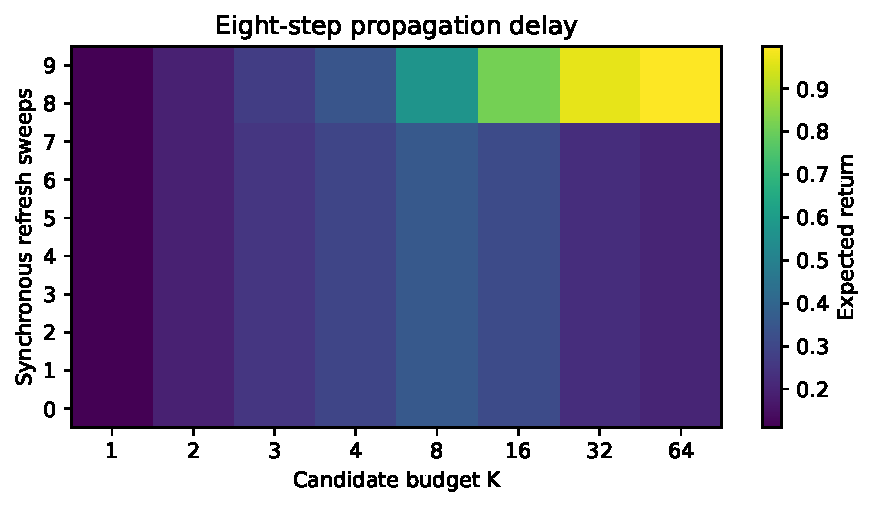
\includegraphics[width=.77\linewidth]{../figures/refresh_heatmap.pdf}
\caption{Depth-eight exact fork. Full sweeps must propagate the changed continuation to the root before its ranking changes. This is a lower bound for synchronous local propagation, not for backward planning.}
\end{figure}
\begin{figure}[t]
\centering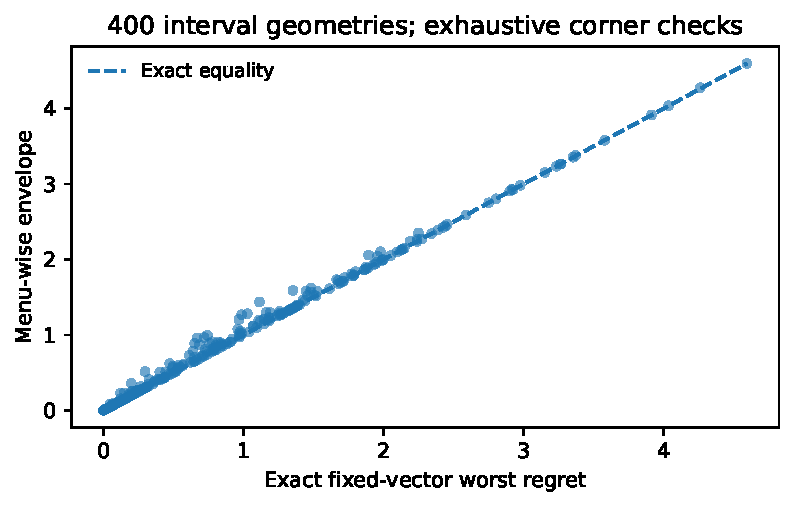
\includegraphics[width=.76\linewidth]{../figures/geometry.pdf}
\caption{The menu-wise envelope versus exhaustive fixed-vector robust regret. Points above the identity are the cost of swapping a supremum and expectation, not a numerical error. The proved factor-four bound is not tight in these tested geometries.}
\end{figure}
\begin{figure}[t]
\centering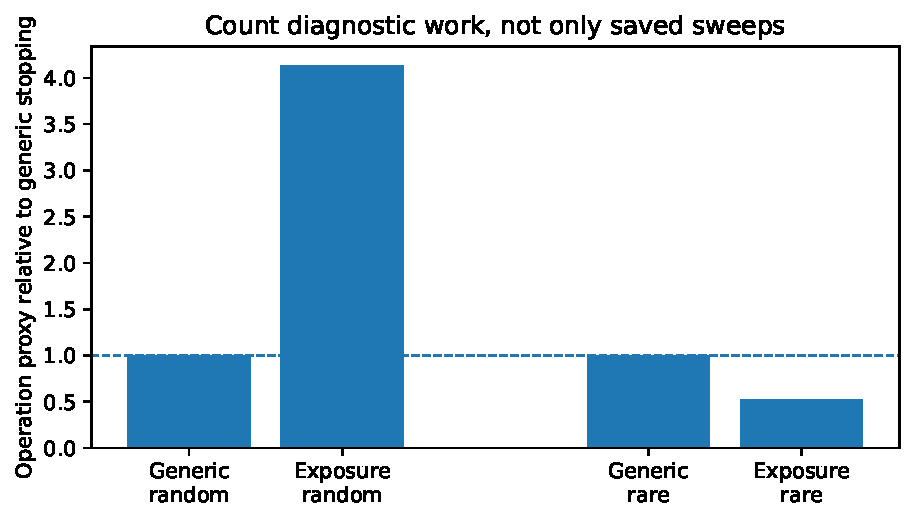
\includegraphics[width=.78\linewidth]{../figures/operation_counts.pdf}
\caption{Complete operation proxy relative to generic stopping. The targeted family benefits, whereas action-rich random graphs are substantially more expensive despite fewer backups.}
\end{figure}

\subsection{Linear critic protocol}
Each layer has a separate weighted ridge regressor. For a layer containing $w$ states and $A$ actions, the features are a bias, $w$ state indicators, $A$ action indicators, and two fixed Gaussian interaction features. The targets are an empirical baseline $Q^\beta$ for initialization and then the empirical expected-max Bellman targets. Sample-count weights are floored at one and normalized to unit mean; the ridge penalty is $.001$. Predictions are clipped to $[0,H-h]$. The regressors never receive oracle $Q_K$ labels. Separate layerwise fitting prevents cross-layer target leakage while leaving low-rank within-layer misspecification. This is a controlled fitted-iteration experiment, not a neural policy benchmark.

\begin{figure}[t]
\centering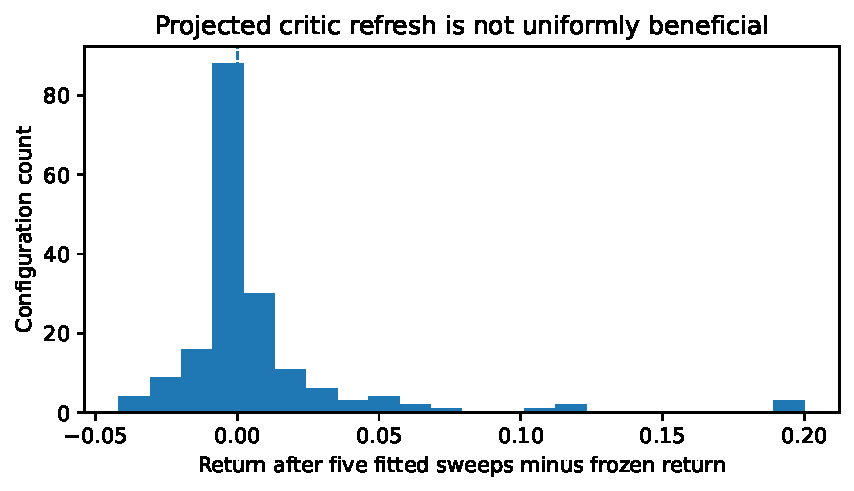
\includegraphics[width=.77\linewidth]{../figures/linear_gains.pdf}
\caption{Return changes after five projected sweeps for 180 task--dataset--budget configurations. Both signs occur. Configurations share tasks and are not 180 independent task-level observations.}
\end{figure}

\subsection{Verification and interpretation}
The test suite checks order-statistic probabilities with ties, large $K$, zero-support actions, exact envelope enumeration, the robust-factor inequalities, shift invariance, the delayed-fork switch, robust transition LPs, residual containment, exact performance-loss propagation, the safe gate, and paid diagnostic accounting. Numerical checks are not formal proof verification. The one observed model-confidence failure in the main 480-dataset grid occurs for the three-layer stochastic family at $N=2000$, seed 13; its presence is retained in the data. No falsely accepted or falsely near-optimal policy is observed there.

The released status note distinguishes completed mathematical arguments and CPU experiments from outstanding external review. The principal open practical issue is whether a cheaper or more structured exposure certificate can retain decision sensitivity without incurring the quadratic cost that dominates our action-rich experiments. A second issue is tighter joint model geometry: rectangular and worst-state bounds discard cancellations that can matter greatly for safe budget transfer.
\end{document}
